\documentclass[12pt]{article}

\usepackage{sbc-template}
\usepackage{graphicx,url}
\usepackage{tikz}
\usetikzlibrary{positioning,fit}
\usepackage[utf8]{inputenc}
\usepackage[english]{babel}
% O template original traz aqui um segundo \usepackage[latin1]{inputenc},
% depois do utf8. Removido: a dupla declaracao quebra a acentuacao.

     
\sloppy

\title{LivreAn\'alise: A Free and Open Source Desktop Tool for\\ Qualitative Data Analysis}

\author{Lucas Tito\inst{1}, Tiago Tito\inst{2},
  Graziella Rodrigues\inst{2}, Jeferson Kenedy M. Vieira\inst{2}}


% TODO confirmar: sua unidade/campus na UPE, e se o Kenedy assina pelo
% Campus Quixada (e como ele assina nos dois artigos da trilha).
% TODO e-mails institucionais dos quatro.
\address{Universidade de Pernambuco (UPE) -- TODO cidade, PE -- Brazil
\nextinstitute
  Campus Quixad\'a -- Universidade Federal do Cear\'a (UFC)\\
  Quixad\'a, CE -- Brazil
  \email{TODO@upe.br,}

  \email{\{TODO,TODO,jefersonkenedy\}@ufc.br}
}

\begin{document} 

\maketitle

\begin{abstract}
  % TODO escrever por ultimo. Maximo 10 linhas.
  % Formula: problema (ferramentas de analise tematica sao pagas) + o que fizemos
  % (ferramenta open source, local, com transcricao de video e export para IA) +
  % resultado (uso em dois TCCs reais, avaliacao com TAM).
\end{abstract}
     
% O bloco \begin{resumo} do template foi removido de proposito: o proprio
% template diz que artigos em ingles apresentam apenas abstract.


\section{Context}

Qualitative coding is a central activity in Information Systems research. The
researcher reads transcripts line by line, assigns codes to excerpts, groups
codes into categories and themes, and revises that structure several times
before arriving at a final set of findings \cite{braun:06}. Doing this by hand,
in a word processor or a spreadsheet, does not scale past a handful of
interviews.

Software support for this activity exists, but it is almost entirely
commercial. The established tools in the field, such as ATLAS.ti, NVivo and
MAXQDA, are proprietary and sold under paid licenses.
% TODO preco e modelo de licenca de cada uma, incluindo licenca de estudante.
% Uma frase com numeros aqui vale mais que o paragrafo inteiro.
This puts them out of reach of a large part of the Brazilian academic
community, and particularly of undergraduate and early graduate students, who
need the tool for a single piece of work and have no funding line to cover it.

The first author faced exactly this problem while writing his undergraduate
thesis. The analysis was carried out in ATLAS.ti, a paid tool, not by
preference but by elimination: the free alternatives available at the time
offered few features and dated interfaces.
% TODO nomear as gratuitas testadas e dizer o que faltou em cada uma.
% Sem isso esta frase e opiniao; com isso vira evidencia.

Beyond cost, two further constraints shaped the problem. First, most
contemporary alternatives are cloud services, which requires uploading research
material to third-party infrastructure. When that material is an interview with
an identifiable participant, this is not a minor operational detail. Second,
none of the tools we examined offered a way to use general-purpose AI
assistants alongside the analysis without handing the entire dataset over to a
model provider.

This paper reports the development of LivreAn\'alise, a free and open source
desktop application for qualitative coding that runs entirely on the
researcher's own machine. Section 2 describes the process and the architecture
adopted, and Section 3 presents the resulting tool and how it has been used so
far.

\section{Adopted Process}

Development started in June 2026 and has followed an iterative and incremental
approach, with four public releases to date; the version described here is
0.7.0, from October 2026. The team is small: two developers, one of whom is the
first author and acts as maintainer, and one supervising researcher. External
contributions are made through pull requests against the public repository, and
roughly a fifth of the commits so far come from a contributor other than the
maintainer.

Three design decisions were taken at the outset and have constrained every
choice since.

\textbf{The application runs locally, with no account and no server.} A project
is a single file on the researcher's disk, so there is no infrastructure to pay
for and no data leaving the machine. This also means the tool works offline.

\textbf{The application embeds no AI model.} Rather than integrating a
provider, which would imply a cost and a data transfer the researcher may not
want, the tool exports the analysis in a form that any external assistant can
read. The integration is manual and deliberate: the researcher decides what
leaves the machine, and when.

\textbf{The project format is interoperable.} Adopting the open REFI-QDA
exchange format \cite{refiqda} means a project can be moved in and out of
ATLAS.ti, so choosing the tool is not a commitment that locks the researcher
in.

The implementation is an Electron application written in TypeScript, with React
and Tailwind in the interface. Project data is stored in SQLite, accessed
through better-sqlite3 and Drizzle, in a single \texttt{.liva} file.
Transcription uses whisper.cpp with quantized Whisper models
\cite{radford:23} in ggml format, and a bundled ffmpeg build extracts the audio
track. Figure~\ref{fig:arquitetura} summarizes the architecture.

% TODO esta figura e TikZ e ainda nao foi compilada. Conferir no primeiro build.
\begin{figure}[ht]
\centering
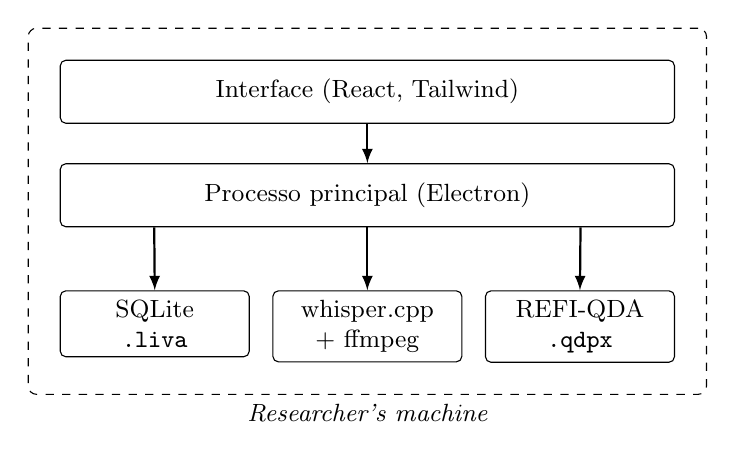
\begin{tikzpicture}[
  font=\small,
  caixa/.style={draw, rounded corners=2pt, minimum height=8mm, align=center,
                inner xsep=4pt},
  seta/.style={-latex, thick}
]
\node[caixa, minimum width=78mm] (ui) {Interface (React, Tailwind)};
\node[caixa, minimum width=78mm, below=5mm of ui] (main)
  {Processo principal (Electron)};
\node[caixa, minimum width=24mm, below=8mm of main.south west, anchor=north west]
  (db) {SQLite\\ \texttt{.liva}};
\node[caixa, minimum width=24mm, below=8mm of main] (whisper)
  {whisper.cpp\\ + ffmpeg};
\node[caixa, minimum width=24mm, below=8mm of main.south east, anchor=north east]
  (qdpx) {REFI-QDA\\ \texttt{.qdpx}};
\draw[seta] (ui) -- (main);
\draw[seta] (main.south west) ++(12mm,0) -- (db.north);
\draw[seta] (main) -- (whisper);
\draw[seta] (main.south east) ++(-12mm,0) -- (qdpx.north);
\node[draw, dashed, rounded corners=3pt, fit=(ui)(main)(db)(whisper)(qdpx),
      inner sep=4mm, label={[font=\small\itshape]below:Researcher's machine}]
      {};
\end{tikzpicture}
\caption{Architecture of LivreAn\'alise. Every component runs locally.}
\label{fig:arquitetura}
\end{figure}

Each merge into the main branch runs the test suite and the type checker and
publishes signed-off installers for Linux, Windows and macOS, so a release is
always reproducible from the repository.

The tool has been evaluated in two ways. It is in use in two ongoing
undergraduate theses, by the second and third authors, who adopted it from the
first public release onwards and whose reports informed successive iterations.
% TODO 1 ou 2 frases com o tema de cada TCC e o volume de material analisado.
A hands-on workshop with a research group outside the development team is also
planned, with an evaluation questionnaire at the end.
% TODO quando a previa da oficina acontecer, substituir esta frase pelo
% resultado: quantos participantes, o que responderam.

\section{Solution}

LivreAn\'alise supports the full coding cycle in a single desktop application.
Documents in \texttt{.docx} and plain text are imported into the project, and
their content is copied into the project file, so moving or deleting the
original afterwards does not break the analysis. The researcher selects an
excerpt and applies a code; coded regions are highlighted in the code's colour
and labelled in the right margin, aligned to where each excerpt begins, as
shown in Figure~\ref{fig:codificacao}. Overlapping codings of the same code are
merged automatically, and the extent of a quotation can be adjusted by dragging
its ends. Documents can be edited inside the application without displacing the
codings already made.

\begin{figure}[ht]
\centering
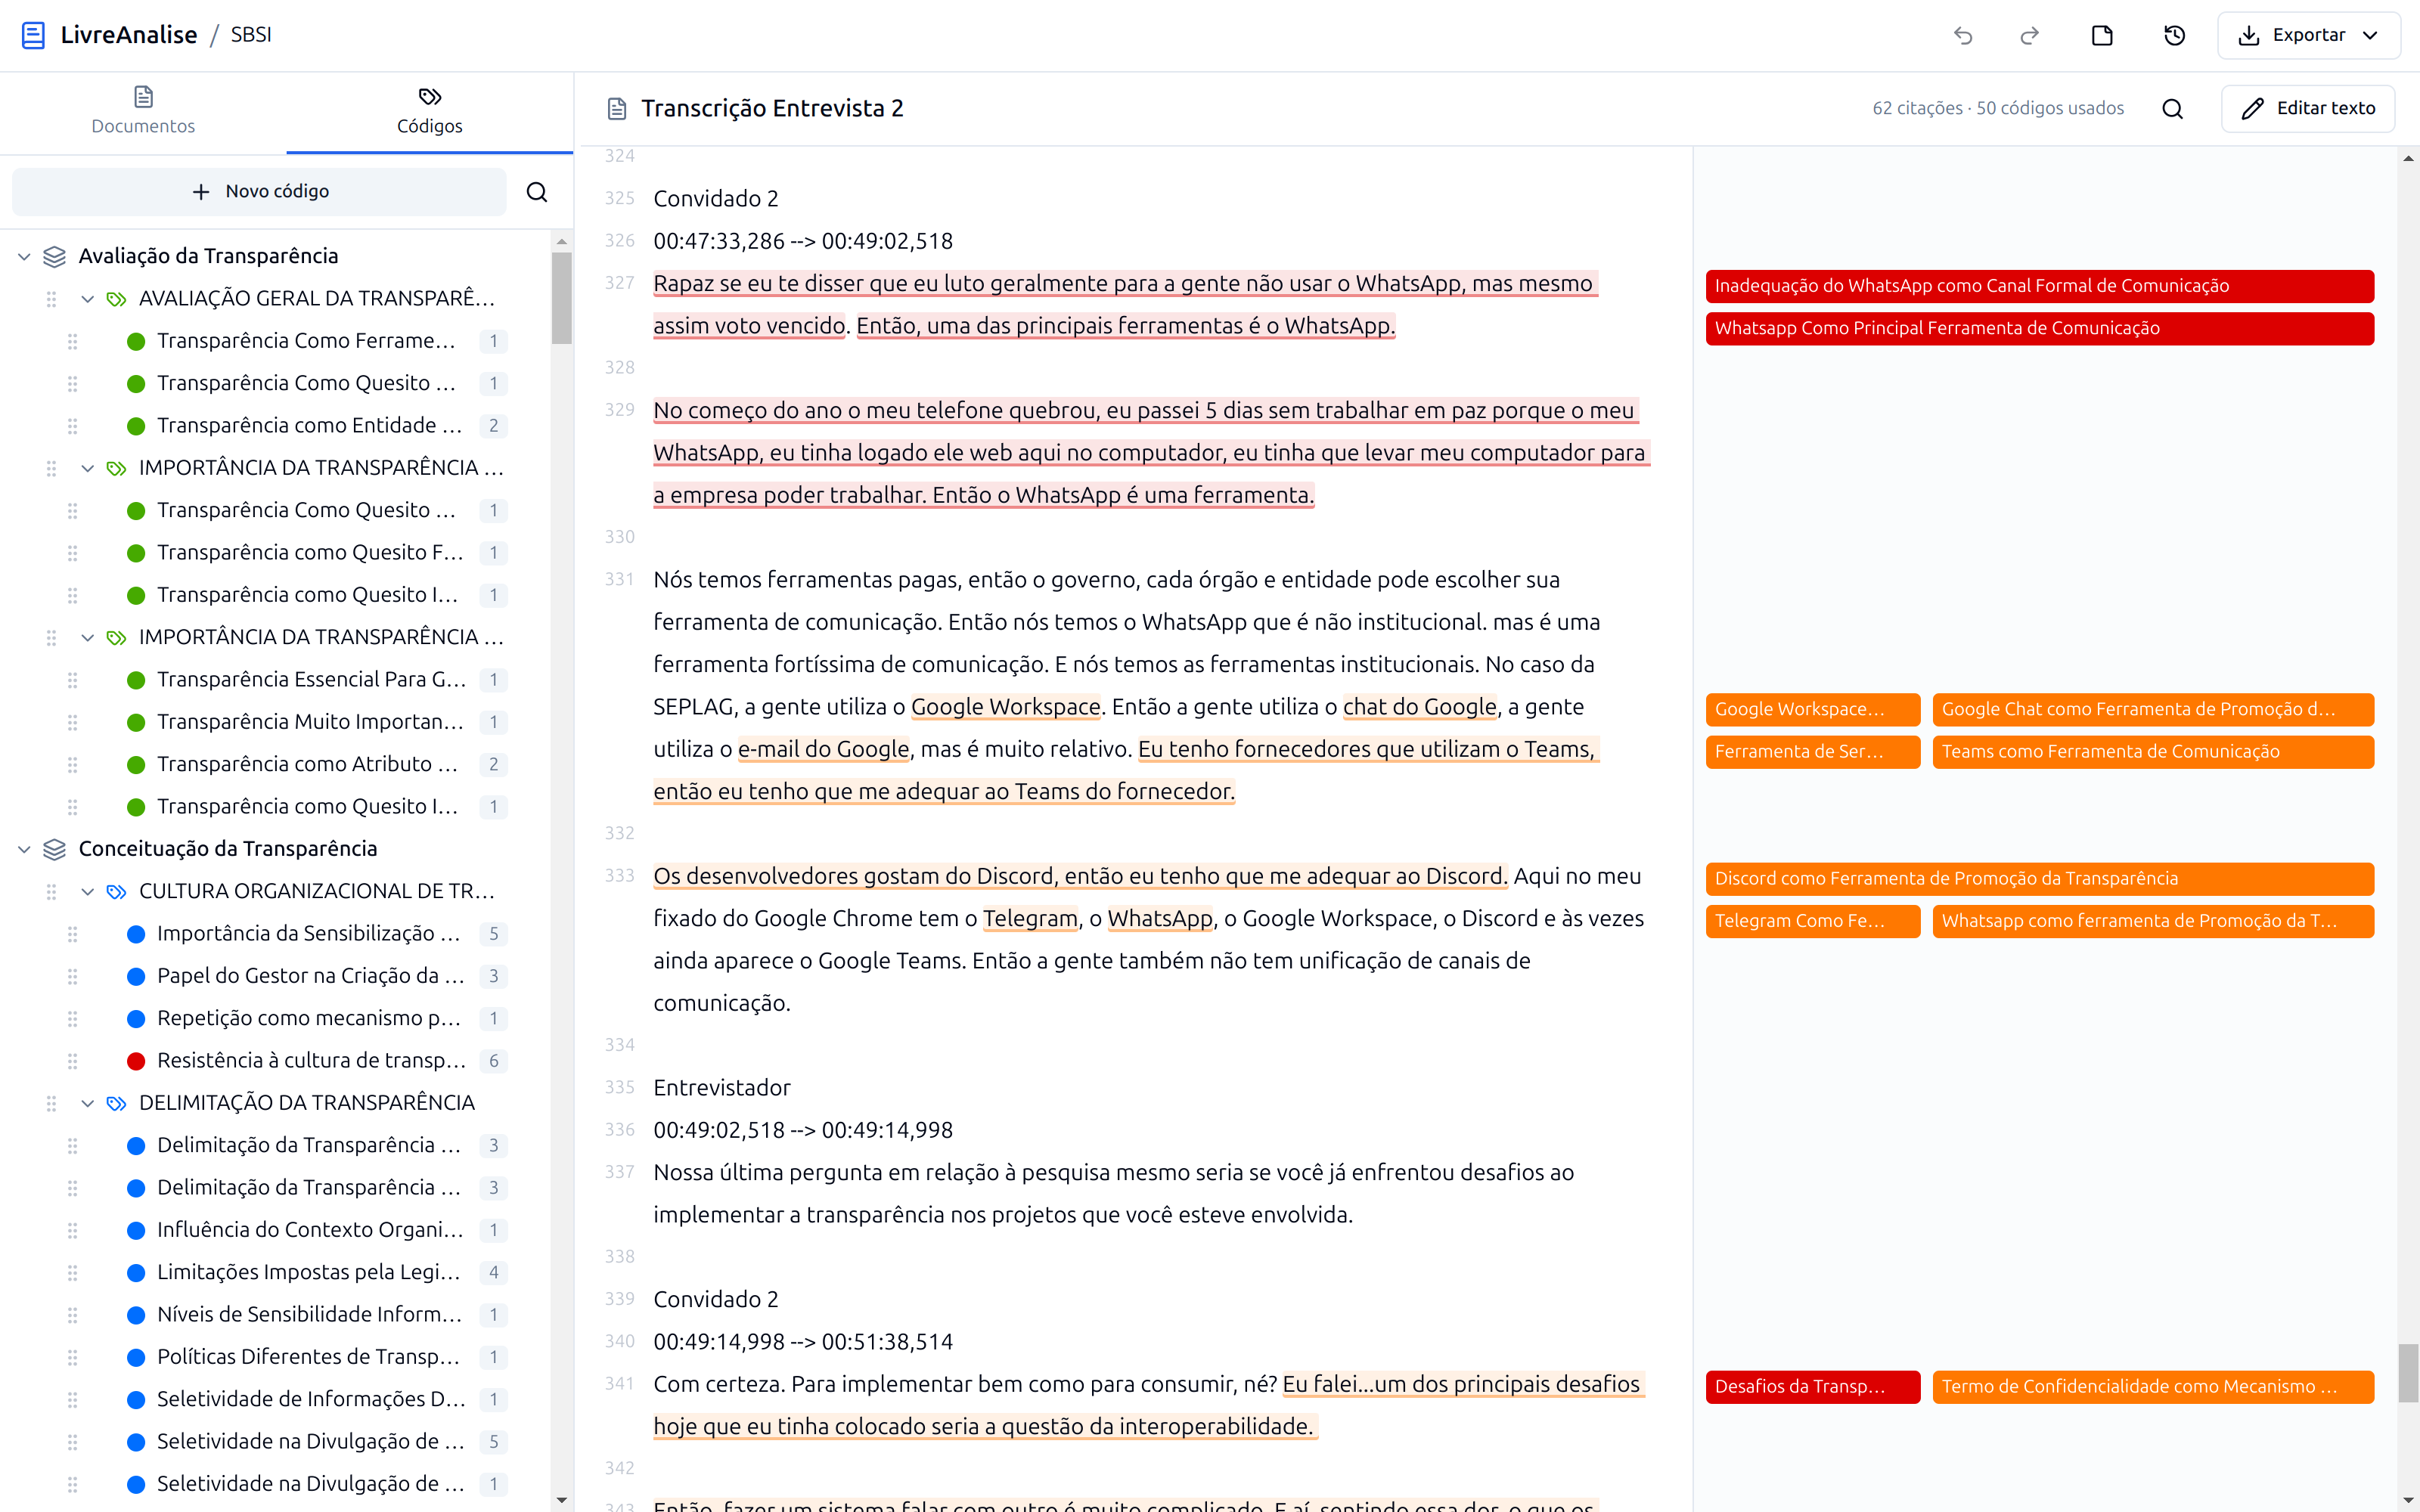
\includegraphics[width=\textwidth]{fig-codificacao.png}
\caption{Coding a document: the hierarchy of groups, categories and codes on
  the left, and the labels aligned on the right margin.}
\label{fig:codificacao}
\end{figure}

The code hierarchy has exactly three levels. A \emph{code} is the atom and the
only level a quotation attaches to. A \emph{category} is a code that contains
other codes, a property derived from having children rather than a separate
kind of entity, and it cannot be applied to an excerpt. A \emph{group} gathers
categories and codes across the hierarchy. Categories and groups are always
created from the items they gather, so a category never exists empty. The tool
also provides per-code usage counts, a list of every excerpt of a given code,
research notes anchored in the text, full undo and redo, named project
checkpoints, search across the project, and typographic settings including the
OpenDyslexic typeface.

Two features distinguish the tool from the free alternatives we found.
Transcription of audio and video runs \textbf{locally}, through whisper.cpp,
with the text appearing on screen as it is recognized and a progress bar driven
by the fraction of audio already processed; nothing is sent to any API. And the
\textbf{AI export} produces a text file describing the analysis at one of three
scopes, from the code structure alone to the full set of documents with their
markings, which the researcher can paste into any assistant. The file opens
with an explicit warning that the material will leave the machine and that
participant consent and ethics approval should be checked first.

Interoperability with ATLAS.ti is provided through REFI-QDA
\cite{refiqda}: a \texttt{.qdpx} project can be opened, creating a new project,
and any project can be exported back. Codes map to leaf \texttt{Code} elements,
categories to nested \texttt{Code} elements, groups to \texttt{Set} and
\texttt{MemberCode}, and quotations to \texttt{PlainTextSelection} and
\texttt{Coding}.

Anonymization is deliberately out of scope. It is the researcher's
responsibility, and the tool expects the material it receives to already be in
the form the research ethics process requires.

The benefits of the approach are threefold. There is \textbf{no cost}, which
removes the barrier that motivated the work. There is \textbf{data
sovereignty}, since no component requires an account, a server or a network
connection, and the material under analysis never leaves the researcher's
machine unless the researcher explicitly exports it. And there is \textbf{no
lock-in}, because the project format is open and the code is public and open to
contribution. The tool is available at
\url{https://github.com/Lucas-Tito/LivreAnalise}.
% TODO fechar a issue #27 antes de submeter: o package.json declara MIT mas nao
% existe arquivo LICENSE, e sem ele o padrao legal e direitos reservados.
% "Open source" e o argumento central deste artigo.

\section*{Acknowledgements}

% TODO se usarem IA generativa para escrever ou revisar, a declaracao e OBRIGATORIA
% pelo Codigo de Conduta para Autores da SBC: listar as ferramentas e dizer onde
% foram empregadas. Pode ficar aqui ou em secao propria.

% ---------------------------------------------------------------------------
% EXEMPLOS DO TEMPLATE SBC, mantidos comentados para copiar quando precisar.
%
% Figura (legenda de uma linha fica centralizada):
% \begin{figure}[ht]
% \centering
% \includegraphics[width=.5\textwidth]{fig1.jpg}
% \caption{A typical figure}
% \label{fig:exampleFig1}
% \end{figure}
%
% Tabela (a legenda vem ANTES da tabela):
% \begin{table}[ht]
% \centering
% \caption{Variables to be considered on the evaluation of interaction techniques}
% \label{tab:exTable1}
% \includegraphics[width=.7\textwidth]{table.jpg}
% \end{table}
%
% Citacao: \cite{knuth:84}, \cite{boulic:91}, \cite{smith:99}
% Referencia cruzada: Section~\ref{sec:figs}, Figure~\ref{fig:exampleFig1}
%
% Regras de formatacao que o template enuncia e o .sty ja aplica:
%  - A4, coluna unica, margens 3,5 cm sup / 2,5 cm inf / 3,0 cm laterais
%  - fonte Times 12 pt, sem cabecalho, sem rodape, sem numero de pagina
%  - titulo de secao em negrito 13 pt, alinhado a esquerda
%  - primeiro paragrafo da secao sem recuo, os seguintes com recuo de 1,27 cm
%  - legendas em Helvetica 10 pt negrito
%  - imagens em preto e branco ou tons de cinza, 600 dpi (PB) ou 150-300 dpi (cinza)
% ---------------------------------------------------------------------------

\bibliographystyle{sbc}
\bibliography{artigo}

\end{document}
